\section{Venn}

\subsection{Venn and the Geometry of Logic: From Boolean Algebra to Statistical Frequency}

Boole gave us the algebra of thought — a symbolic logic to reason under uncertainty. But it was still abstract, opaque, and hard to visualize.

Enter \textbf{John Venn} (1834–1923), the philosopher-mathematician who drew the picture everyone else had only imagined. Venn wasn’t trying to revolutionize mathematics — just to clarify Boole. And yet, in doing so, he gave the world a new visual grammar: the \textbf{Venn diagram}.

Where Boole used equations, Venn used space. Circles for sets. Overlaps for intersections. The absence of overlap for logical negation. With these simple tools, he made logic tangible — and turned abstract reasoning into spatial intuition.

\begin{figure}[H]
    \centering
    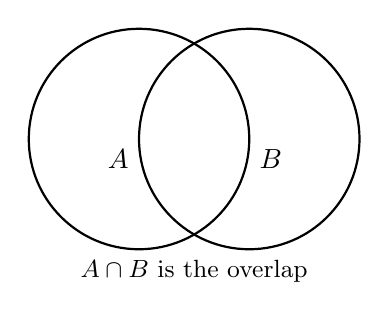
\begin{tikzpicture}[scale=1.4]
        \draw[thick] (0,0) circle (1) node[below left] {$A$};
        \draw[thick] (1,0) circle (1) node[below right] {$B$};
        \node at (0.5,-1.2) {\small $A \cap B$ is the overlap};
    \end{tikzpicture}
    \caption{A basic Venn diagram: Logic rendered as geometry.}
\end{figure}

But Venn didn’t stop at visual logic. He was also deeply engaged with the foundations of probability — and here, he made a move that quietly set the stage for modern statistics.

\subsection{Probability as Long-Run Frequency}

While Laplace treated probability as **epistemic** (a measure of belief), and Boole treated it as an extension of logic, Venn argued for a different interpretation:  
\textbf{Probability is not a state of mind — it is a fact about the world.}

In his 1866 work, *The Logic of Chance*, Venn rejected subjective and metaphysical definitions of probability. Instead, he framed probability as an empirical phenomenon — something that arises from **relative frequency over repeated trials**.

\begin{quote}
\textit{“It is to the statistics of large numbers of instances that we must look, and not to the supposed ‘reasonableness’ of single judgments.”} \\
— \textbf{John Venn}, *The Logic of Chance*
\end{quote}

This was a major philosophical shift: probability was no longer about ignorance or belief. It became about data — the measurable outcome of real-world repetitions. Where Laplace dealt in symmetry and Boole in possibility, Venn dealt in actual, observed regularity.

\subsection{The Concept of Empirical Structure}

Venn’s frequency interpretation introduced a new layer of structure. He accepted that outcomes might be uncertain, but insisted that they were not unknowable. Given enough trials, the probabilities would reveal themselves — not as truths we impose, but as patterns that emerge.

This idea — that statistical truth lives in the **long run**, and that theory must meet observation — would become a cornerstone of scientific inference. And while Venn didn’t yet build the full machinery of statistics, he handed the tools to someone who would.

\begin{quote}
\textit{If Boole gave logic a symbolic form, and Venn gave it shape, then it was Fisher who gave it power.}
\end{quote}

\medskip

In the next section, we’ll see how \textbf{Ronald Fisher} transformed Venn’s frequency-based vision into a precision toolkit — one capable of estimating parameters, testing hypotheses, and extracting structure from randomness.

\begin{tcolorbox}[colback=gray!5!white, colframe=black!75!white, title={Historical Sidebar: John Stuart Mill and the Logic of Observation}]

    \textbf{John Stuart Mill} (1806–1873) was a philosopher, political economist, and logician whose fingerprints are all over 19th-century British thought — including the statistical philosophy of John Venn.
    
    While earlier thinkers like Descartes sought certainty through reason alone, Mill insisted that knowledge comes from experience. In his landmark 1843 treatise, \emph{A System of Logic}, Mill argued that all scientific reasoning must be grounded in \textbf{empirical observation} — in what we actually see, not just what we can imagine.
    
    Mill’s method was inductive. Truths emerge not from deduction, but from patterns that persist across repeated trials. He laid out “canons” of experimental reasoning — principles for identifying cause and effect from regularities in data.
    
    \medskip
    
    \textbf{This is exactly the spirit Venn adopted.} In rejecting Laplace’s symmetry-based probability and Boole’s logical idealism, Venn leaned hard into Mill’s worldview: that the structure of truth is revealed in frequencies, not formulated in the abstract.
    
    \begin{quote}
    \emph{“Probability is not what we reason about — it is what the world shows us, again and again.”}
    \end{quote}
    
    This empirical turn would ripple through the next century. It shaped Fisher’s statistics, Popper’s falsifiability, and even modern machine learning. But it started with Mill — and Venn was listening.
    
\end{tcolorbox}
